\documentclass{article}
\usepackage{amsmath}
\usepackage{amssymb}
\usepackage{amsthm}
\usepackage{mathabx}
\usepackage{graphicx}
\usepackage{hyperref}
\usepackage{listings}
\usepackage{xcolor}
\usepackage{fp}[nomessages]
\usepackage{tikz}

\setlength{\parindent}{0pt}

\usetikzlibrary{fit}
\usetikzlibrary{arrows}

\lstset { %
	language=C++,
	backgroundcolor=\color{black!5}, % set backgroundcolor
	basicstyle=\footnotesize,% basic font setting
}

\graphicspath{{./graphics/}}

\newtheorem{theorem}{Theorem}[section]
\newtheorem{corollary}{Corollary}[theorem]
\newtheorem{lemma}{Lemma}[theorem]
\newtheorem{definition}{Definition}[section]
\newtheorem*{remark}{Remark}

\title{Notes for NTT, version 0.2}
\author{Antti Roeyskoe}
\date{31.5.2019}

\begin{document}
\begin{titlepage}
\maketitle
\end{titlepage}

\newpage

\section{Number-Theoretic Transform}
\subsection{Goal}
Given a prime $p$ and integer $d$ such that $d = 2^{k}$ for some $k$ and $2^{k+1} \divides p-1$, and two polynomials $P$ and $Q$
\begin{align*}
P(x) &= \sum_{i = 0}^{d-1} a_{i} x^{i}\\
Q(x) &= \sum_{i = 0}^{d-1} b_{i} x^{i}\\
\end{align*}
The algorithm finds the remainders mod $p$ of the coefficients $c_{i}$ of the product polynomial $R(x) = P(x)Q(x)$:
\begin{align*}
R(x)		&= \sum_{i = 0}^{2d-1} c_{i} x^{i}\\
		&= \sum_{i = 0}^{2d-1} \left(\sum_{j = 0}^{i} a_{j}b_{i-j}\right) x^{i}\\
		&= P(x)Q(x)
\end{align*}
where $a_{j}$ and $b_{j}$ are zero for terms that don't exist ($j < 0$ or $d \leq j$)

\subsection{Intuition}
Define vectors
\begin{align*}
a &= [a_{0}, \dots, a_{d-1}, 0, \dots, 0]\\
b &= [b_{0}, \dots, b_{d-1}, 0, \dots, 0]\\
c &= [c_{0}, \dots, c_{2d-1}]\\
\end{align*}
of length $2d$.

Let $x$ be some integer. Let $M$ be a $2d \times 2d$ matrix where $M_{i,j} = x^{ij}$ (zero-indexed).

Now
\begin{align*}
aM	&= [P(x^{0}), \dots, P(x^{2d-1})]\\
bM	&= [Q(x^{0}), \dots, Q(x^{2d-1})]\\
\end{align*}
(proof in appendix) and
\begin{align*}
cM	&= [R(x^{0}), \dots, R(x^{2d-1})]\\
	&= [P(x^{0})Q(x^{0}), \dots, P(x^{2d-1})Q(x^{2d-1})]\\
	&= aM \circ bM
\end{align*}
Where $\circ$ is the elementwise matrix product.

We will choose $x$ such that $M^{-1}$ exists, and then get
\begin{align*}
c	&= cMM^{-1}\\
	&= (aM \circ bM)M^{-1}
\end{align*}
So if we can calculate $vM$ and $vM^{-1}$ for a vector $v$ in time $O(n \log n)$, we can calculate $c$ from $a$ and $b$ in $O(n \log n)$.
It turns out that this is possible! But first we need some number-theoretic background.

\subsection{Number-Theoretic Background}
Let $p$ be a prime. Let $P$ to denote the group $\mathbb{Z}/p\mathbb{Z}$ of integers mod $p$. 

\begin{definition}
The order $ord(g)$ of an element $g \in P$ is the minimum positive integer such that $g^{ord(g)} \equiv 1 \text{ mod } p$.
\end{definition}
\begin{definition}
An element $g \in P$ a generator if $ord(g) = p-1$
\end{definition}

Let $g \in P, g \not\equiv 0$ be some nonzero element mod $p$. The following statements are true:
\begin{itemize}
	\item $g^{p-1} \equiv 1 \text{ mod } p$ (fermat's little theorem)
	\item If $g^{a} \equiv 1 \text{ mod } p$, then $ord(g) \divides a$.
	\item If $b \divides ord(g)$, then $ord(g^{b}) = \frac{ord(g)}{b}$.
	\item For odd primes, exactly $\frac{p-1}{2}$ elements in $P$ are generators.
	\item If $g$ is a generator of $p$, then $\frac{1}{p}$ is also a generator of $p$.
	\item If $ord(g) = 2$, $g \equiv -1 \text{ mod } p$.
\end{itemize}
(proof in the appendix)

\subsection{Algorithm}
Recall that we require $d = 2^{k}$ for some integer $k$, and that $2^{k+1} \divides p-1$.

Let $g \in P$ be a generator. For any $n \divides 2^{k}$, set $x_{n} \equiv g^{\frac{p-1}{n}} \text{ mod } p$, and let $M[n]$ be a $n \times n$ matrix where
\begin{equation*}
M[n]_{i,j} \equiv x_{n}^{ij} \text{ mod } p
\end{equation*}
Note that this $M[n]$ is of the wanted type with $x = x_{n}$. It turns out that $M[n]^{-1}$ exists, and that we can calculate $vM[n]$ fast. Next we'll show how:

\subsubsection{Forward Direction}

Let $n$ be some power of two such that $n \divides 2^{k}$. Let $v = [v_{0}, \dots, v_{n-1}]$, $v_{i} \in P$ be a vector with length $n$.
Define $f(v): v \mapsto vM[n]$. We'll now show how to compute $f(v)$ in time $O(n \log n)$.

If $n = 1$, then since $x_{1} \equiv 1$, $vM[n] = [v_{0}]$. When $n > 1$, define
\begin{align*}
even(v) &= [v_{0}, v_{2}, \dots, v_{n-2}]\\
odd(v) &= [v_{1}, v_{3}, \dots, v_{n-1}]\\
\end{align*}
(note that $n$ is a power of two greater than $1$, so it is even.) Let $0 \leq j < n$ be some index, and define $h = \frac{n}{2}$. we have
\begin{align*}
(vM[n])_{j}	&\equiv \sum_{i=0}^{n-1} v_{i} M[n]_{i, j}\\
		&\equiv \sum_{i=0}^{n-1} v_{i} x_{n}^{ij}\\
		&\equiv \sum_{i=0}^{h-1} v_{2i} x_{n}^{2ij} + \sum_{i=0}^{h-1} v_{2i+1} x_{n}^{(2i+1)j}\\
		&\equiv \sum_{i=0}^{h-1} v_{2i} \left(x_{n}^{2}\right)^{ij} + x_{n}^{j} \sum_{i=0}^{h-1} v_{2i+1} \left(x_{n}^{2}\right)^{ij} \text{ mod } p\\
\end{align*}

We have $x_{n}^{2} = x_{h}$ by definition:
\begin{align*}
x_{n}^{2}	&\equiv \left(g^{\frac{p-1}{n}}\right)^{2}\\
		&\equiv g^{2 \frac{p-1}{n}}\\
		&\equiv g^{\frac{p-1}{h}}\\
		&\equiv x_{h} \text{ mod } p
\end{align*}

therefore
\begin{align*}
(vM[n])_{j}	&\equiv \sum_{i=0}^{h-1} v_{2i} \left(x_{n}^{2}\right)^{ij} + x_{n}^{j} \sum_{i=0}^{h-1} v_{2i+1} \left(x_{n}^{2}\right)^{ij}\\
		&\equiv \sum_{i=0}^{h-1} v_{2i} x_{h}^{ij} + x_{n}^{j} \sum_{i=0}^{h-1} v_{2i+1} x_{h}^{ij} \text{ mod } p\\
\end{align*}

If $j < h$, then
\begin{align*}
(vM[n])_{j}	&\equiv \sum_{i=0}^{h-1} v_{2i} x_{h}^{ij} + x_{n}^{j} \sum_{i=0}^{h-1} v_{2i+1} x_{h}^{ij}\\
		&\equiv f(even(v))_{j} + x_{n}^{j} f(odd(v))_{j} \text{ mod } p\\
\end{align*}

If $j \geq h$, We have
\begin{equation*}
1 \equiv 1^{i} \equiv x_{1}^{i} \equiv \left(x_{h}^{h}\right)^{i} \equiv x_{h}^{ih} \text{ mod } p
\end{equation*}
Set $j^{'} = j - h$. Now $0 \leq j^{'} < h$, so
\begin{align*}
(vM[n])_{j}	&\equiv (vM[n])_{j^{'} + h}\\
		&\equiv \sum_{i=0}^{h-1} v_{2i} x_{h}^{i(j^{'} + h)} + x_{n}^{j^{'} + h} \sum_{i=0}^{h-1} v_{2i+1} x_{h}^{i(j^{'} + h}\\
		&\equiv \sum_{i=0}^{h-1} v_{2i} x_{h}^{ij^{'}} x_{h}^{ih} + x_{n}^{j^{'} + h} \sum_{i=0}^{h-1} v_{2i+1} x_{h}^{ij^{'}} x_{h}^{ih}\\
		&\equiv \sum_{i=0}^{h-1} v_{2i} x_{h}^{ij^{'}} + x_{n}^{j^{'} + h} \sum_{i=0}^{h-1} v_{2i+1} x_{h}^{ij^{'}}\\
		&\equiv f(even(v))_{j^{'}} + x_{n}^{j^{'} + h} f(odd(v))_{j^{'}}\\
		&\equiv f(even(v))_{j^{'}} + x_{n}^{h} x_{n}^{j^{'}} f(odd(v))_{j^{'}}\\
		&\equiv f(even(v))_{j^{'}} - x_{n}^{j^{'}} f(odd(v))_{j^{'}} \text{ mod } p\\
\end{align*}
Since $ord\left(x_{n}^{h}\right) = 2$, and therefore $x_{n}^{h} \equiv -1 \text { mod } p$.

Therefore for $0 \leq j < h$ we have:
\begin{align*}
(vM[n])_{j}	&\equiv f(even(v))_{j} + x_{n}^{j} f(odd(v))_{j}\\
(vM[n])_{j+h}	&\equiv f(even(v))_{j} - x_{n}^{j} f(odd(v))_{j}\\
\end{align*}
So when we have $f(even(v))$ and $f(odd(v))$, we can easily calculate $f(v)$ in linear time. Since $even(v)$ and $odd(v)$ have size $h = \frac{n}{2}$,
we can calculate them recursively. This gives a $O(n log n)$ algorithm.

\subsubsection{Reverse Direction}

To find $M[n]^{-1}$, note that we only used the fact that $g$ is a generator. But $\frac{1}{g}$ is also a generator.
Set $g^{'} = \frac{1}{g}$, and define $M^{'}[n]$ similarly as how $M[n]$ is defined, except that it uses $g^{'}$ instead of $g$.
We have
\begin{equation*}
M[n]M^{'}[n] = nI[n]
\end{equation*}
(proof in the appendix) Where $I[n]$ is the identity matrix of size $n \times n$. Therefore $\frac{1}{n} M^{'}[n]$ is the inverse matrix of $M[n]$.
Furthermore, we have
\begin{equation*}
v \left(\frac{1}{n} M^{'}[n]\right) = \left(v \frac{1}{n}\right) M^{'}[n]
\end{equation*}
So we can multiply a vector with $\frac{1}{n} M^{'}[n]$ the same way as we multiplied it with $M[n]$, just by changing the generator we give to the function.

\section{Code and Improvements}
\subsection{Recursive Code}
All codes will have the same includes and definitions. Here we define the prime and generator we will be using.
\begin{lstlisting}
#include <iostream>
#include <vector>
using namespace std;
using ll = long long;
const int P = 998244353; // 2^21 | P-1
const int G = 3; // 3 is a generator of P
\end{lstlisting}

The main NTT-function. It modifies the input vector instead of building a new one.
\begin{lstlisting}
void ntt(vector<int>& v, int x_n) {
	int h = v.size()/2;
	vector<int> even(h);
	vector<int> odd(h);
	for (int i = 0; i < h; ++i) {
		even[i] = v[2*i];
		odd[i] = v[2*i+1];
	}

	if (h > 1) {
		int x_h = (ll)x_n*x_n % P;
		ntt(even, x_h);
		ntt(odd, x_h);
	}

	ll mult = 1; // (x_n)^i
	for (int i = 0; i < h; ++i) {
		v[i] = (even[i] + mult * odd[i]) % P;
		v[i+h] = (even[i] - mult * odd[i]) % P;
		if (v[i+h] < 0) v[i+h] += P;
		mult = mult*x_n % P;
	}
}
\end{lstlisting}
Here we have the usual function for calculating $a^{b} \text{ mod } P$, and a helper function
wrapping the calls to NTT made when multiplying two polynomials $a$ and $b$. If vectors $a$ and $b$
contain the coefficients $a[i] = a_{i}$, $b[i] = b_{i}$ of polynomials $A$ and $B$, then the result
vector $c$ will contain the coefficients $c[i] = c_{i}$ of $C = AB$.
\begin{lstlisting}
ll modPow(ll a, ll b) {
	if (b & 1) return a * modPow(a, b-1) % P;
	if (b == 0) return 1;
	return modPow(a*a % P, b / 2);
}

vector<int> polyMult(const vector<int>& a, const vector<int>& b) {
	int as = a.size();
	int bs = b.size();
	int n = 1;
	while(n < (as + bs)) n <<= 1;
	int x_n = modPow(G, (P-1)/n);
	int inv_x_n = modPow(x_n, P-2);
	int inv_n = modPow(n, P-2);

	vector<int> ap (n, 0);
	vector<int> bp (n, 0);
	for (int i = 0; i < as; ++i) ap[i] = a[i] % P;
	for (int i = 0; i < bs; ++i) bp[i] = b[i] % P;
	
	ntt(ap, x_n);
	ntt(bp, x_n);

	vector<int> cp(n);
	for (int i = 0; i < n; ++i) {
		ll prod = (ll)ap[i] * bp[i] % P;
		cp[i] = prod * inv_n % P;
	}

	ntt(cp, inv_x_n);

	cp.resize(as + bs - 1);
	return cp;
}
\end{lstlisting}

\subsection{Iterative Code}
TODO

\section{Tricks with NTT}
\subsection{Number of Paths}
A common problem is that we want to calculate the number of paths from some source cell $(x_{s}, y_{s})$ to other cells in a grid,
such that at every step we can move from $(x, y)$ to $(x+1, y)$ or $(x, y+1)$, and there are some blocked cells we cannot enter.

Given a square with side length $n$ containing no blocked cells, and how many ways exist to get from the source to each cell on the left side
or on the bottom side of the square, we want to calculate the number of ways to get from the source to cells on the top side and right side of the square.

This is possible since any path from the source cell to a cell in the square must travel through its left or bottom side. To calculate the number of ways
to reach the top and right sides, we can use simple $O(n^{2})$ dp, setting $ways[x][y] = (ways[x-1][y] + ways[x][y-1]) \% P$.

\begin{figure}[]
\begin{center}
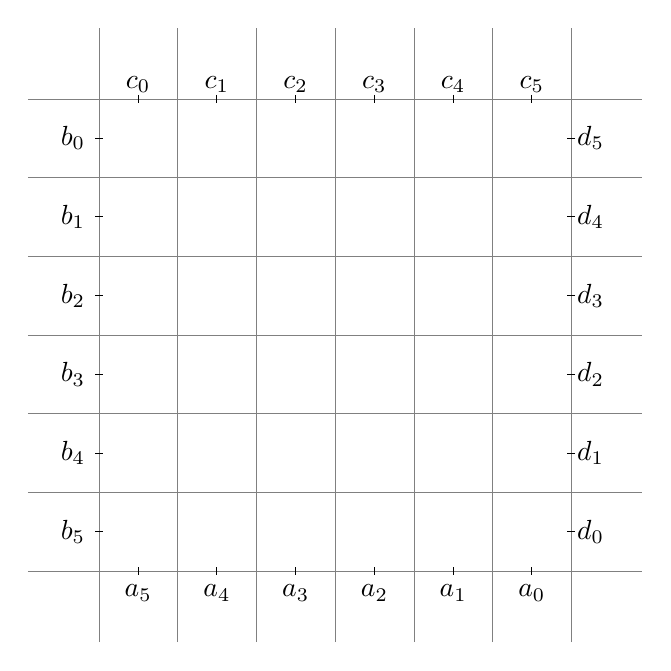
\begin{tikzpicture}[]
	\draw[step=1cm,gray,very thin] (-0.9,-0.9) grid (6.9, 6.9);
	\foreach \i in {0,1,2,3,4,5}
		\def\x{\the\numexpr-\i+5.5}
		\draw (\x cm,0.05cm) -- (\x cm,-0.05cm) node[anchor=north] {$a_{\i}$};
	\foreach \i in {0,1,2,3,4,5}
		\def\x{\the\numexpr\i+0.5}
		\draw (\x cm,6.05cm) -- (\x cm,5.95cm) node[anchor=south] {$c_{\i}$};
	\foreach \i in {0,1,2,3,4,5}
		\def\y{\the\numexpr-\i+5.5}
		\draw (0.05cm,\y cm) -- (-0.05 cm,\y cm) node[anchor=east] {$b_{\i}$};
	\foreach \i in {0,1,2,3,4,5}
		\def\y{\the\numexpr\i+0.5}
		\draw (6.05cm,\y cm) -- (5.95cm,\y cm) node[anchor=west] {$d_{\i}$};
\end{tikzpicture}
\caption{Indexing of the arrays. The arrays $a, b$ are the input arrays, and $c, d$ the output arrays.}
\end{center}
\end{figure}
\begin{figure}[]
\begin{center}
\begin{tikzpicture}[]
	\draw[step=2cm,gray,very thin] (-1.9,-1.9) grid (5.9, 5.9);
	\foreach \i in {0,1}
		\def\x{\the\numexpr-\i*2+3}
		\draw (\x cm,0.05cm) -- (\x cm,-0.05cm) node[anchor=north] {$a_{\i}$};
	\foreach \i in {0,1}
		\def\x{\the\numexpr\i*2+1}
		\draw (\x cm,4.05cm) -- (\x cm,3.95cm) node[anchor=south] {$c_{\i}$};
	\foreach \i in {0,1}
		\def\y{\the\numexpr-\i*2+3}
		\draw (0.05cm,\y cm) -- (-0.05 cm,\y cm) node[anchor=east] {$b_{\i}$};
	\foreach \i in {0,1}
		\def\y{\the\numexpr\i*2+1}
		\draw (4.05cm,\y cm) -- (3.95cm,\y cm) node[anchor=west] {$d_{\i}$};
	\node[] at (-1cm, 1cm) {$1$};
	\node[] at (-1cm, 3cm) {$3$};
	\node[] at (1cm, -1cm) {$0$};
	\node[] at (1cm, 1cm) {$1$};
	\node[] at (1cm, 3cm) {$4$};
	\node[] at (1cm, 5cm) {$4$};
	\node[] at (3cm, -1cm) {$1$};
	\node[] at (3cm, 1cm) {$2$};
	\node[] at (3cm, 3cm) {$6$};
	\node[] at (3cm, 5cm) {$6$};
	\node[] at (5cm, 1cm) {$2$};
	\node[] at (5cm, 3cm) {$6$};
\end{tikzpicture}
\caption{Example values and ways to reach the positions. Note that $c_{n-1} = d_{n-1}$,
since they both represent the number of ways to reach the up-right corner.}
\end{center}
\end{figure}

If $P$ is a suitable prime for $NTT$, this can be done faster, in time $O(n \log n)$.

Let $c1[j]$ be the vector representing the number of ways to get from the source to $c_{j}$ through some node in $a$,
and $c2[j]$ respectively be the number of ways to get from the source to $c_{j}$ through some node in $b$. Note that every
path is counted exactly once among these two, so $c[j] = c1[j] + c2[j]$.

We have
\begin{align*}
c1[j] &= \sum_{i = n-1-j}^{n-1} a[i] \binom{i+j}{n-1}\\
c2[j] &= \sum_{i = 0}^{n-1} b[i] \binom{i+j}{j}\\
\end{align*}

So these can be calculated with the following matrix multiplications:
\begin{align*}
aM1 &= a\left[\begin{array}{ccccc}
	0			&\dots	&0			&\dots	&\binom{n-1}{n-1}\\
	\vdots			&	&\vdots			&	&\vdots\\
	0			&\dots	&\binom{i+j}{n-1}	&\dots	&\binom{n-1+i}{n-1}\\
	\vdots			&	&\vdots			&	&\vdots\\
	\binom{n-1}{n-1}	&\dots	&\binom{n-1+j}{n-1}	&\dots	&\binom{2n-2}{n-1}\\
\end{array}\right] = c1\\
bM2 &= b\left[\begin{array}{ccccc}
	\binom{0}{0}	&\dots	&\binom{j}{j}		&\dots	&\binom{n-1}{n-1}\\
	\vdots		&	&\vdots			&	&\vdots\\
	\binom{i}{0}	&\dots	&\binom{i+j}{j}		&\dots	&\binom{n-1+i}{n-1}\\
	\vdots		&	&\vdots			&	&\vdots\\
	\binom{n-1}{0}	&\dots	&\binom{n-1+j}{j}	&\dots	&\binom{2n-2}{n-1}\\
\end{array}\right] = c2\\
\end{align*}
Changing the second to factorials we get
\begin{align*}
M2	&= \left[\begin{array}{ccccc}
	\frac{0!}{0!0!}		&\dots	&\frac{j!}{j!0!}		&\dots	&\frac{(n-1)!}{(n-1)!0!}\\
	\vdots			&	&\vdots				&	&\vdots\\
	\frac{i!}{0!i!}		&\dots	&\frac{(i+j)!}{j!i!}		&\dots	&\frac{(n-1+i)!}{(n-1)!i!}\\
	\vdots			&	&\vdots				&	&\vdots\\
	\frac{(n-1)!}{0!(n-1)!}	&\dots	&\frac{(n-1+j)!}{j!(n-1)!}	&\dots	&\binom{(2n-2)!}{(n-1)!(n-1)!}\\
\end{array}\right]\\
	&= diag\left(\begin{bmatrix}
	\frac{1}{0!}\\
	\vdots\\
	\frac{1}{i!}\\
	\vdots\\
	\frac{1}{(n-1)!}\\
	\end{bmatrix}\right)\ M3\ diag\left(\begin{bmatrix}
	\frac{1}{0!}\\
	\vdots\\
	\frac{1}{i!}\\
	\vdots\\
	\frac{1}{(n-1)!}\\
	\end{bmatrix}\right)\\
\end{align*}
Where $diag$ makes a diagonal matrix with the elements of the vector on the diagonal, and
\begin{equation*}
M3 = \left[\begin{array}{ccccc}
	0!	&\dots	&j!		&\dots	&(n-1)!\\
	\vdots	&	&\vdots		&	&\vdots\\
	i!	&\dots	&(i+j)!		&\dots	&(i+n-1)!\\
	\vdots	&	&\vdots		&	&\vdots\\
	(n-1)!	&\dots	&(n-1+j)!	&\dots	&(2n-2)!\\
	\end{array}\right]
\end{equation*}

Note that we can multiply a vector with a diagonal matrix in $O(n)$, and that both $M1$ and $M3$ have the form
\begin{equation*}
\left[\begin{array}{ccccc}
	x_{0}	&\dots	&x_{j}		&\dots	&x_{n-1}\\
	\vdots	&	&\vdots		&	&\vdots\\
	x_{i}	&\dots	&x_{i+j}	&\dots	&x_{i+n-1}\\
	\vdots	&	&\vdots		&	&\vdots\\
	x_{n-1}	&\dots	&x_{n-1+j}	&\dots	&x_{2n-2}\\
	\end{array}\right]
\end{equation*}

Matrices in this form are called Hankel matrices. We'll later show how to multiply a vector with a matrix in this form in $O(n \log n)$ time using NTT.

So now we just calculate $c = c1 + c2$ in $O(n \log n)$ time with two FFT-calls. $d$ is symmetric, swapping $a$ and $b$. We just need to calculate the values
$\binom{k}{n-1}$ and $k!$ for $0 \leq k < 2n-1$. But $\binom{k}{n-1} = \frac{k!}{(n-1)!k!}$, so it is enough to precalculate the values and modular inverses
of $0 \leq k < 2n-1$. This can be done in $O(n \log n)$ time by calculating inverses with the extended euclidean algorithm, assuming we can do arithmetic
operations on numbers up to $P$ in $O(1)$ time.

\subsubsection{Multiplying vectors with Hankel matrices}
We want to multiply a vector $v = [v_{0}, \dots, v_{n-1}]$ with the Hankel matrix
\begin{equation*}
M = \left[\begin{array}{ccccc}
	x_{0}	&\dots	&x_{j}		&\dots	&x_{n-1}\\
	\vdots	&	&\vdots		&	&\vdots\\
	x_{i}	&\dots	&x_{i+j}	&\dots	&x_{i+n-1}\\
	\vdots	&	&\vdots		&	&\vdots\\
	x_{n-1}	&\dots	&x_{n-1+j}	&\dots	&x_{2n-2}\\
	\end{array}\right]
\end{equation*}
To do this, we use NTT on the vectors $v^{'} = [v_{0}, \dots, v_{n-1}, 0, \dots, 0]$, $x^{'} = [x_{2n-2}, \dots, x_{0}]$
of length $2n-1$. For $0 \leq i < n$, the $2n-2-i$th entry of the result will be:
\begin{align*}
NTT(v^{'}, x^{'})_{2n-2-i}	&= \sum_{j = 0}^{2n-2-i} v^{'}_{j} x^{'}_{2n-2-i-j}\\
				&= \sum_{j = 0}^{n-1} v_{j} x^{'}_{2n-2 - (i+j)}\\
				&= \sum_{j = 0}^{n-1} v_{j} x_{i+j}\\
				&= (vM)_{i}
\end{align*}
So we can set $res_{i} = NTT(v^{'}, x^{'})_{2n-2-i}$ for $0 \leq i < n$

\section{appendix}
TODO

\end{document}
